\documentclass[11pt]{article}
\usepackage[margin=1in]{geometry}
\usepackage[T1]{fontenc}
\usepackage{lmodern,textcomp}
\usepackage{amsmath,amssymb,booktabs,graphicx,float,xcolor}
\usepackage[round,authoryear]{natbib}
\usepackage[hidelinks]{hyperref}

\newcommand{\E}{\mathbb{E}}
\newcommand{\1}{\mathbf{1}}
\renewcommand{\arraystretch}{1.12}
\setlength{\abovecaptionskip}{4pt}
\setlength{\belowcaptionskip}{6pt}

\title{Do Tail-Risk Models Add Value Beyond Volatility and Correlation?\\
\large Evidence from Multi-Asset Markets}
\author{Shangrong Li\thanks{Research note, not peer reviewed. Code and data-retrieval notebooks:
\url{https://github.com/lshangro-png/tail-risk-cn}. All results can be regenerated from free public data sources.}}
\date{October 2026}

\begin{document}
\maketitle

\begin{abstract}
\noindent
Tail-risk methods (copula tail dependence, expected shortfall budgeting) are widely promoted in sell-side
research as improvements over volatility- and correlation-based risk management. This note asks whether they
carry information that volatility and correlation do not. Two tests are run on Chinese and global asset
classes. \emph{Test 1} compares tail-dependence statistics with a Gaussian-copula null that matches the
observed correlation matrix in every estimation block. Single-parameter Clayton/Gumbel coefficients, the
quantities used in practice, are statistically indistinguishable from this null: their rank correlation with
the ordinary correlation is 0.94 in the data and 0.94 under the null. Models with a separate tail parameter
do detect dependence beyond correlation in a six-asset weekly panel (31 of 105 Student-$t$ versus Gaussian
tests reject at 5\%, against 5.7 expected under the matched null), concentrated in risky-asset pairs and in the
lower tail; between Chinese stocks and government bonds the evidence is weak and has no downside asymmetry.
\emph{Test 2} decomposes tail risk parity into its two ingredients: replacing volatility by expected
shortfall, and conditioning on GARCH volatility forecasts. Replacing volatility by ES adds 0.00--0.04 to the
excess Sharpe ratio, never significantly. Conditioning adds about 0.11 before costs, but raises annual
one-way turnover from 15\% to 95\%, and the gain is gone at 25 basis points per unit traded. A preliminary
section shows that the Acerbi--Szekely $Z_2$ threshold of $-0.70$, calibrated for 250 observations, is
uninformative in long backtests, and replaces it with a self-normalised test with a wild-bootstrap $p$-value.
Within the markets and sample studied, the incremental value of these tail-risk methods over tracking current
volatility and correlation is small.
\end{abstract}

% ---------------------------------------------------------------------------
\section{Introduction}

Volatility and linear correlation describe a multivariate return distribution only up to its second moments.
Tail-risk methods promise more: copula tail-dependence coefficients are meant to capture joint crashes that
correlation misses \citep{embrechts2002}, and expected shortfall (ES) is a coherent measure of the loss beyond
the value-at-risk (VaR). Chinese sell-side reports have turned these ideas into trading rules, for example a
stock--bond ``double-kill'' warning triggered by rolling Clayton and Gumbel tail coefficients, hierarchical
allocation on lower-tail distances, and tail risk parity \citep{alankar2013}. The question this note asks is
narrow: \emph{given current volatility and correlation, do these tail-risk statistics add information?}

Two difficulties make the question harder than it looks. First, the natural benchmark is not independence.
A single-parameter Archimedean copula fitted to positively correlated data returns a positive tail coefficient
even when the true copula is Gaussian and has no tail dependence. The null has to hold the correlation fixed.
Second, an allocation built on ES may differ from one built on volatility for two separate reasons: the risk
measure changes, and the scenarios used to estimate it are often conditioned on current volatility. These two
effects have to be separated, and the comparison has to be made net of the turnover each one generates.

The note makes three contributions. (i)~It runs a \emph{correlation-matched} Gaussian-copula null for a
panel of tail-dependence statistics, which handles both the correlation confound and the dependence between
tests that share an asset. (ii)~It decomposes tail risk parity into a $2\times 2$ design (risk measure $\times$
conditioning) and evaluates it under two explicit execution rules with realised turnover and transaction
costs. (iii)~It shows that the fixed $Z_2$ threshold commonly used to backtest ES is not calibrated for long
samples and gives a simple replacement.

The underlying replications of sell-side reports, with their code, are in the accompanying repository. This
note summarises the two strongest lines of evidence from that work.

% ---------------------------------------------------------------------------
\section{Data}

All data come from free public sources: the ChinaBond website (bond wealth indices), Sina, Tencent and
Eastmoney via AkShare (Chinese indices and ETFs), FRED (exchange rates, Brent, volatility indices) and the
Kenneth French library. Prices are stored in a local SQLite database and every result is recomputed from it.

\begin{itemize}
\item \textbf{Single-asset backtests (Section~\ref{sec:marginal}).} Daily returns of the SSE 50, CSI 300 and
CSI 500 indices, the ChinaBond composite wealth index, gold (GLD $\times$ USD/CNY), the S\&P 500 and Brent,
from 1987--2006 (depending on the series) to October 2026.
\item \textbf{Stock--bond pair (Section~\ref{sec:test1}).} CSI 300 and ChinaBond composite wealth index,
daily, 2003--2026. Both close at the same time in Beijing.
\item \textbf{Multi-asset panel (Section~\ref{sec:test1}) and allocation (Section~\ref{sec:test2}).}
CSI 300, CSI 500, S\&P 500, ChinaBond government-bond total wealth index (CGB), gold in CNY and Brent.
Chinese and Western markets close at different times, which biases same-day dependence towards zero, so the
dependence tests use \emph{weekly} (Friday-to-Friday) returns. The allocation backtest is monthly and uses
daily returns from 2005 to October 2026 (5{,}008 common trading days).
\item \textbf{ETF panel.} Ten Chinese-listed ETFs (domestic equity styles, Nasdaq, Hang Seng, gold,
commodities), 2016--2026, used for the lower-tail-distance comparison.
\end{itemize}

% ---------------------------------------------------------------------------
\section{Preliminary: marginal tails and a calibrated ES backtest}
\label{sec:marginal}

Before testing dependence, it is worth checking what matters for one asset at a time. Six one-day-ahead
VaR/ES forecasters are run on rolling 1{,}000-day windows: historical simulation, Gaussian, Student-$t$,
GPD peaks-over-threshold, GJR-GARCH(1,1) with filtered historical simulation (FHS), and GJR-GARCH with a GPD
tail on the standardised residuals \citep[GARCH-EVT;][]{mcneil2000,glosten1993}. The 99\% VaR is evaluated
with the \citet{kupiec1995} unconditional-coverage test and the \citet{christoffersen1998} independence test,
and the 97.5\% ES with the $Z_2$ statistic of \citet{acerbi2014}.

\paragraph{The $Z_2$ test needs a null distribution, not a fixed threshold.}
Let $X_t$ be the return, $\mathrm{VaR}_t$ and $\mathrm{ES}_t$ the forecasts at level $\alpha$ (both positive
numbers), and $I_t = \1\{X_t < -\mathrm{VaR}_t\}$. Acerbi and Szekely define
\begin{equation}
Z_2 = \frac{1}{T\alpha}\sum_{t=1}^{T}\frac{X_t I_t}{\mathrm{ES}_t} + 1 .
\end{equation}
Write $Y_t = X_t I_t/\mathrm{ES}_t + \alpha$, so $Z_2 = \sum_t Y_t/(T\alpha)$. If both forecasts are correct,
$\E_{t-1}[X_t I_t] = -\alpha\,\mathrm{ES}_t$, hence $\E_{t-1}[Y_t]=0$: $\{Y_t\}$ is a martingale-difference
sequence, whatever the volatility dynamics. Acerbi and Szekely report $-0.70$ as an approximate 5\% critical
value, obtained by simulation with $T=250$. The null standard deviation of $Z_2$ shrinks like
$1/\sqrt{T\alpha}$, so in a backtest of $T\approx 5{,}000$ days a fixed $-0.70$ corresponds to a far smaller
test size and much lower power. I therefore use the self-normalised statistic
\begin{equation}
S = \frac{\sum_t Y_t}{\sqrt{\sum_t Y_t^2}} \xrightarrow{d} N(0,1)\quad\text{under } H_0,
\end{equation}
which follows from the martingale central limit theorem \citep{hallheyde1980}. A finite-sample $p$-value is
obtained by a wild bootstrap: $S^{*} = \sum_t Y_t\varepsilon_t/\sqrt{\sum_t Y_t^2}$ with independent
Rademacher $\varepsilon_t$ \citep{wu1986,mammen1993}. The test is one-sided: a significantly negative $S$
means the ES is too small or VaR violations are too frequent. A related cumulative-violation approach is
\citet{duescanciano2017}.

\paragraph{Monte Carlo check.}
Table~\ref{tab:z2mc} simulates a GARCH(1,1) with standardised $t_5$ innovations
($\omega=0.02$, $\alpha=0.08$, $\beta=0.90$, returns in percent) and evaluates three forecasts of the 97.5\%
ES: the true conditional VaR and ES; a Gaussian tail with the true volatility, which understates ES by 14\%
while VaR is only 1.6\% too low; and the true forecasts scaled by 0.85. With $T=250$ the rule $Z_2<-0.70$
rejects the correct model in 5.3\% of samples, as designed. With $T=5{,}000$ it never rejects the correct
model, never detects the Gaussian tail, and detects the 15\% scaling in only 37\% of samples. The test on $S$
has size 4.3\% at $T=5{,}000$ and power of 62\% and 100\% against the two misspecifications. At $T=250$
the asymptotic test is conservative (size 1.7\%; a year contains only about six 97.5\% violations), and
the wild-bootstrap $p$-value should be used. In the long backtests below, asymptotic and bootstrap $p$-values
agree to within 0.03.

\begin{table}[t]
\centering
\caption{Rejection rates of the 97.5\% ES backtest in 1{,}000 simulations of a GARCH(1,1) with standardised $t_5$ innovations. ``Rule'': $Z_2<-0.70$. ``Test'': one-sided asymptotic test on $S$ at 5\%.}
\label{tab:z2mc}
\small
\begin{tabular}{lrrrr}
\toprule
 & \multicolumn{2}{c}{$T=250$} & \multicolumn{2}{c}{$T=5000$} \\ \cmidrule(lr){2-3}\cmidrule(lr){4-5}
Forecast & Rule & Test & Rule & Test \\
\midrule
Correct model & 5.3\% & 1.7\% & 0.0\% & 4.3\% \\
Gaussian tail, correct volatility & 15.7\% & 4.5\% & 0.0\% & 61.5\% \\
VaR and ES scaled by 0.85 & 44.5\% & 25.3\% & 37.0\% & 100.0\% \\
\bottomrule
\end{tabular}
\end{table}


\paragraph{Results.}
Table~\ref{tab:var} reports, for each method, the number of the seven assets for which each test
does not reject at 5\%. With the fixed threshold, the Gaussian model ``passes'' the ES backtest for six of
seven assets, although its realised tail losses exceed the forecast ES by 27\% (median). With the
calibrated test it is rejected for all seven. Methods without volatility updating (historical simulation,
Student-$t$, GPD) have roughly correct unconditional coverage, but their violations cluster: the
probability of a violation on the day after a violation is 4--15\% instead of 1\%, and the
Christoffersen test rejects for six of seven assets. Their ES is rejected for three to five assets. Both GARCH
filters pass all three tests for nearly every asset; adding a GPD tail to the filtered residuals (GARCH-EVT)
improves clustering slightly over FHS (6/7 versus 5/7).

\begin{table}[t]
\centering
\caption{One-day-ahead VaR/ES backtests on seven assets (rolling 1{,}000-day windows). Columns 3--6 count the assets (of 7) for which the test does not reject at 5\%. ``Old rule'': $Z_2>-0.70$. ``Calibrated'': one-sided wild-bootstrap $p$-value of the self-normalised statistic $S$. Last column: median over assets of mean realised loss over mean forecast ES on 97.5\% VaR violation days.}
\label{tab:var}
\small
\resizebox{\linewidth}{!}{\begin{tabular}{lrrrrrr}
\toprule
Method & 99\% VaR hit rate & Kupiec & Christoffersen & $Z_2$ old rule & $Z_2$ calibrated & Loss/ES \\
\midrule
Historical simulation & 1.22\% & 5/7 & 1/7 & 7/7 & 4/7 & 1.03 \\
Gaussian & 1.83\% & 0/7 & 0/7 & 6/7 & 0/7 & 1.27 \\
Student-$t$ & 1.13\% & 3/7 & 1/7 & 7/7 & 2/7 & 1.00 \\
GPD (POT) & 1.12\% & 5/7 & 1/7 & 7/7 & 4/7 & 1.03 \\
GARCH-FHS & 1.07\% & 7/7 & 5/7 & 7/7 & 7/7 & 1.03 \\
GARCH-EVT & 0.97\% & 7/7 & 6/7 & 7/7 & 7/7 & 1.03 \\
\bottomrule
\end{tabular}}
\end{table}


The lesson for what follows is that, at the level of a single asset, the information that matters is the
current volatility. Tail-shape modelling on top of a GARCH filter (EVT versus FHS) changes little.

% ---------------------------------------------------------------------------
\section{Test 1: tail dependence beyond correlation}
\label{sec:test1}

\subsection{Why single-parameter tail coefficients mostly measure correlation}

The Clayton copula $C_\theta(u,v) = (u^{-\theta}+v^{-\theta}-1)^{-1/\theta}$ has lower tail dependence
$\lambda_L = 2^{-1/\theta}$; the Gumbel copula has $\lambda_U = 2-2^{1/\theta}$. Each family has one
parameter, which governs both the overall strength of positive dependence and the tail. When either is fitted
to data whose true copula is Gaussian with correlation $\rho>0$, maximum likelihood moves $\theta$ away from
the independence boundary to match the overall dependence, and $\hat\lambda$ becomes positive although the
true tail dependence is zero \citep{joe1997}. The appropriate null is therefore a Gaussian copula with the
same correlation, not independence.

On the CSI 300--ChinaBond pair, with rolling 60-day windows as in the CICC (2021) warning rule, this matters a
great deal. In a Gaussian copula with $\rho=0.3$, 94\% of 60-day windows already give $\hat\lambda_L>0$ under
the point-estimate rule. The 60-day correlation alone separates days with $\hat\lambda_L>0$ from days with
$\hat\lambda_L=0$ with an AUC of 0.95. Against a Gaussian null that matches each window's normal-score
correlation, the observed frequency of $\hat\lambda_L>0$ is 33.4\% versus 34.5\% expected, and the frequency
of the CICC trigger ($\hat\lambda_L>0$, $\hat\lambda_U=0$) is 4.8\% versus 4.7\%. The signal is what
time-varying correlation produces on its own. In the ten-ETF panel, the rank correlation between pairwise
Clayton $\hat\lambda_L$ (250-day windows) and the ordinary correlation averages 0.98 across rebalancing dates,
and a portfolio-ES aggregation formula using $\hat\lambda_L$ is no more accurate than one using $\rho$
(median absolute error 2.2\% versus 2.0\%).

\subsection{Models with a separate tail parameter}

To ask whether there is tail dependence \emph{beyond} correlation, the model needs a parameter for the tail
that is separate from the one for overall dependence. Two are used.

\emph{Student-$t$ versus Gaussian copula.} The $t$ copula has correlation $\rho$ and degrees of freedom $\nu$;
its tail dependence $\lambda = 2\,t_{\nu+1}\!\left(-\sqrt{(\nu+1)(1-\rho)/(1+\rho)}\right)$ vanishes as
$\nu\to\infty$, where it becomes Gaussian \citep{demarta2005}. With the same $\rho$, a finite $\nu$ means extremes
occur together more often than the Gaussian copula implies. The likelihood-ratio statistic for $H_0:\nu=\infty$
lies on the boundary of the parameter space, so its null distribution is
$\tfrac12\chi^2_0+\tfrac12\chi^2_1$ and $p=\tfrac12 P(\chi^2_1\ge \mathrm{LR})$.

\emph{Symmetrised Joe--Clayton (SJC) copula} \citep{patton2006}. Its two parameters are the lower and upper
tail-dependence coefficients $\tau_L,\tau_U$, so $H_0:\tau_L=\tau_U$ is a one-restriction likelihood-ratio
test of tail asymmetry.

For the stock--bond pair, the $t$ test is run in each calendar year (non-overlapping windows, so rejections
can be counted with a binomial test). It rejects Gaussianity at 5\% in 4 of 23 years against 1.15 expected
(binomial $p=0.026$), and in 7 of 22 years after scaling returns by trailing 60-day volatility ($p=10^{-4}$).
The implied tail dependence is small (median 0.2\% over rolling 250-day windows). The direction is symmetric:
both assets fall into their worst 10\% on the same day 57 times and into their best 10\% 55 times, against
47.5 expected under the Gaussian copula. The SJC test finds no downside asymmetry (pooled $p=0.79$ over the
five years with any measurable tail dependence). Between Chinese stocks and government bonds, the dependence
beyond correlation is weak and does not favour joint crashes.

\subsection{A multi-asset panel with a correlation-matched null}

The stock--bond pair is one pair. I extend the tests to all 15 pairs of the six allocation assets, in seven
non-overlapping three-year blocks of weekly returns (2005--2025, 139--153 weeks per block), giving 105
pair-blocks. Within a block, ranks are converted to pseudo-observations and, for each pair, I record the $t$
versus Gaussian $p$-value, the $t$-implied $\lambda$, the SJC estimates and asymmetry $p$-value, the Clayton
$\hat\lambda_L$, and the number of weeks in which both assets fall into their lowest (highest) decile.

\paragraph{Null.} Tests that share an asset are dependent, so the number of rejections is not binomial, and
the $t$ test is mildly oversized for strongly correlated pairs (8\% at $\rho=0.6$ with 156 observations).
Both problems are handled by simulating the whole panel under the null. In each block, the null is a
six-dimensional Gaussian copula whose correlation matrix equals the block's normal-score correlation matrix.
It therefore reproduces the cross-sectional correlation structure and its variation across blocks, and has no
tail dependence. Data of the same length are simulated, every statistic is recomputed exactly as for the
observed data, and the procedure is repeated 200 times. Each summary statistic is compared with its simulated
null distribution, with one-sided $p$-values $(1+\#\{s^*\ge s\})/(1+200)$.

\begin{table}[t]
\centering
\caption{Multi-asset panel (6 assets, 15 pairs, 7 non-overlapping three-year blocks of weekly returns, 105 pair-blocks) against the correlation-matched Gaussian-copula null (200 simulations). $p$: one-sided simulated $p$-value (large values of the statistic). Volatility-scaled: returns divided by trailing 26-week volatility.}
\label{tab:panel}
\small
\resizebox{\linewidth}{!}{\begin{tabular}{lrrrrrr}
\toprule
 & \multicolumn{3}{c}{Raw weekly returns} & \multicolumn{3}{c}{Volatility-scaled} \\ \cmidrule(lr){2-4}\cmidrule(lr){5-7}
Statistic & Obs. & Null mean [5\%, 95\%] & $p$ & Obs. & Null mean & $p$ \\
\midrule
\# $t$ vs Gaussian rejections (5\%) & 31 & 6 [1, 10] & 0.005 & 31 & 6 & 0.005 \\
Mean $t$-implied $\lambda$ & 0.063 & 0.018 [0.010, 0.028] & 0.005 & 0.064 & 0.018 & 0.005 \\
Joint lower-decile weeks & 302 & 235 [212, 257] & 0.005 & 299 & 226 & 0.005 \\
Joint upper-decile weeks & 251 & 231 [207, 257] & 0.104 & 226 & 224 & 0.438 \\
Lower $-$ upper & 51 & 4 [-25, 32] & 0.015 & 73 & 3 & 0.005 \\
Mean SJC $\hat\tau_L-\hat\tau_U$ & 0.049 & 0.000 [-0.016, 0.018] & 0.005 & 0.055 & 0.001 & 0.005 \\
\# SJC asymmetry rejections (5\%) & 8 & 2 [0, 5] & 0.005 & 7 & 2 & 0.010 \\
Mean Clayton $\hat\lambda_L$ & 0.096 & 0.082 [0.073, 0.093] & 0.015 & 0.094 & 0.079 & 0.020 \\
Spearman($\hat\lambda_L,\rho$) & 0.94 & 0.94 [0.92, 0.96] & 0.512 & 0.94 & 0.94 & 0.413 \\
\bottomrule
\end{tabular}}
\end{table}


\begin{figure}[t]
\centering
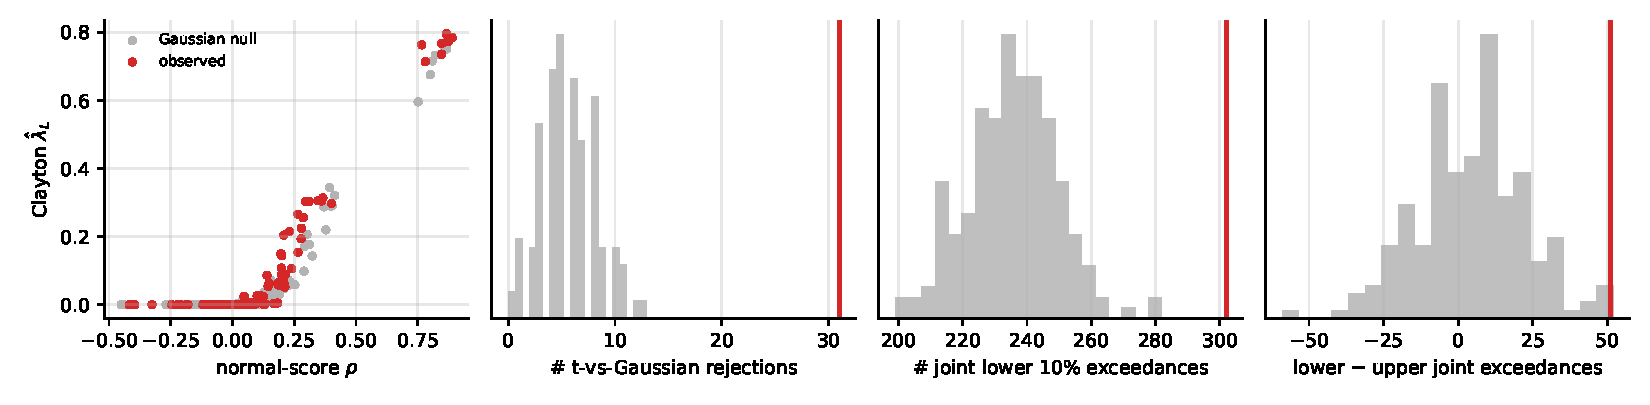
\includegraphics[width=\textwidth]{figures/fig_panel.pdf}
\caption{Multi-asset panel, raw weekly returns. Left: Clayton $\hat\lambda_L$ against the normal-score
correlation for the 105 pair-blocks (red) and for one simulation of the matched Gaussian null (grey). Other
panels: null distributions (grey) of three summary statistics and the observed value (red line).}
\label{fig:panel}
\end{figure}

Table~\ref{tab:panel} and Figure~\ref{fig:panel} give two clear answers.

\emph{The Clayton coefficient carries no information beyond correlation.} Its rank correlation with $\rho$ is
0.94 in the data and 0.94 under the null; the mean $\hat\lambda_L$ is only slightly higher than under the null
(0.096 versus 0.082). Whatever tail dependence exists, the statistic used by the sell-side rules is almost
entirely a monotone function of correlation.

\emph{There is tail dependence beyond correlation, and it is stronger in the lower tail.} The $t$ test rejects in 31
of 105 pair-blocks against 5.7 expected under the matched null ($p<0.01$). Joint lower-decile weeks exceed
joint upper-decile weeks by 51, against 4 under the null ($p=0.015$), and SJC estimates have
$\tau_L>\tau_U$ on average. Scaling returns by their trailing 26-week volatility, which removes common
volatility regimes, leaves these results unchanged or slightly stronger. The $t$-test rejections are spread
across many pairs, including some involving government bonds. The lower-tail excess, however, comes from pairs of
risky assets: S\&P 500--Brent (29 joint lower-decile weeks against 18 upper), gold--Brent (26 against 13) and
CSI 300--S\&P 500 (26 against 16). Pairs involving government bonds show no lower-tail excess.

So the answer to Test 1 depends on the statistic. Tail dependence beyond correlation is statistically
detectable in weekly data, with a lower-tail excess among risky assets. It is not visible in the single-parameter coefficients used in
practice, and between Chinese equities and bonds, the pair that most stock--bond warning rules target, it is
small and symmetric.

% ---------------------------------------------------------------------------
\section{Test 2: does ES risk budgeting add value?}
\label{sec:test2}

\subsection{Design}

Risk parity chooses long-only weights $w$ so that each asset's contribution to a risk measure $R$ is equal.
For a positively homogeneous $R$, the equal-risk-contribution portfolio is $w=y^*/\mathbf{1}'y^*$, with
\begin{equation}
y^* = \arg\min_{y>0}\; R(y) - \sum_{i=1}^{n} b_i\log y_i ,\qquad b_i = 1/n,
\end{equation}
a convex problem whenever $R$ is convex \citep{spinu2013,maillard2010}. For volatility,
$R(y)=\tfrac12 y'\Sigma y$ (the quadratic form, which yields the same solution as $\sqrt{y'\Sigma y}$).
For ES at level $q$ on scenarios $x_1,\dots,x_T$, the \citet{rockafellar2000} representation gives a linear
program inside the objective:
\begin{equation}
R(y) = \min_{a,\;u\ge 0}\; a + \frac{1}{(1-q)T}\sum_{t=1}^{T}u_t \quad\text{s.t.}\quad u_t\ge -x_t'y - a .
\end{equation}
This formulation keeps all ES contributions positive and equal at the optimum even when a hedge asset has a
negative contribution at equal weights, a case where fixed-point iterations fail \citep{mausser2018}.

Four strategies form a $2\times 2$ design:

\begin{center}
\begin{tabular}{lcc}
\toprule
 & Unconditional scenarios & Conditional (FHS) scenarios \\
\midrule
Volatility budget & RP & Conditional RP \\
ES budget ($q=95\%$) & TRP (historical) & Conditional TRP \\
\bottomrule
\end{tabular}
\end{center}

Unconditional scenarios are the last 500 daily returns. Conditional scenarios are the same returns filtered
by a univariate GJR-GARCH(1,1) per asset and rescaled to tomorrow's forecast volatility (multivariate FHS,
\citealp{baroneadesi1999}). This keeps the historical cross-sectional dependence of the residuals and
updates the scale. The ES effect is the row difference, holding the scenarios fixed; the conditioning effect
is the column difference.

\paragraph{Execution and costs.} Target weights are computed at each month end and become effective at the
next open. Two execution rules are evaluated, both tracking actual holdings day by day: \emph{daily
rebalancing} back to target (a constant-mix strategy), and \emph{monthly rebalancing with buy-and-hold}, in
which weights drift with prices between rebalancing dates. On each trading day the amount traded is
$\sum_i|w_{i,t}^{\text{target}}-w_{i,t^-}|$, where $w_{t^-}$ are the drifted holdings, and a cost of
$c\in\{0,10,25,50\}$ basis points per unit traded is deducted from that day's return. Annual one-way turnover
is half the annualised amount traded. Differences in excess Sharpe ratios (risk-free rate 2\%) are assessed
with a moving-block bootstrap (blocks of 20 days, 2{,}000 resamples; \citealp{kunsch1989}), which preserves
volatility clustering; see \citet{ledoit2008} for the same problem with HAC inference.

\subsection{Results}

\begin{table}[t]
\centering
\caption{Tail risk parity decomposition, July 2007 to October 2026, monthly targets from 500-day windows. Turnover is realised annual one-way turnover. Excess Sharpe ratios (risk-free rate 2\%) under monthly rebalancing with buy-and-hold, net of the cost per unit traded shown in the column header.}
\label{tab:trp}
\footnotesize
\resizebox{\linewidth}{!}{\begin{tabular}{lrrrrrr}
\toprule
 & \multicolumn{2}{c}{Turnover} & \multicolumn{4}{c}{Excess Sharpe, cost per unit traded} \\ \cmidrule(lr){2-3}\cmidrule(lr){4-7}
Strategy & Daily & Monthly & 0 bp & 10 bp & 25 bp & 50 bp \\
\midrule
RP & 53\% & 15\% & 0.93 & 0.92 & 0.91 & 0.89 \\
TRP (historical) & 54\% & 16\% & 0.97 & 0.96 & 0.95 & 0.92 \\
Conditional RP & 136\% & 95\% & 1.04 & 0.99 & 0.91 & 0.77 \\
Conditional TRP & 134\% & 95\% & 1.06 & 1.00 & 0.92 & 0.77 \\
\midrule
\multicolumn{7}{l}{\emph{Differences in excess Sharpe, monthly buy-and-hold: estimate [95\% block-bootstrap interval]}} \\
\multicolumn{3}{l}{ES effect (conditional scenarios)} & +0.02 [-0.06, +0.09] & +0.01 [-0.06, +0.09] & +0.01 [-0.06, +0.08] & 0.00 [-0.07, +0.07] \\
\multicolumn{3}{l}{ES effect (unconditional)} & +0.04 [-0.02, +0.11] & +0.04 [-0.03, +0.10] & +0.04 [-0.03, +0.10] & +0.03 [-0.03, +0.10] \\
\multicolumn{3}{l}{Conditioning effect (volatility)} & +0.11 [-0.07, +0.30] & +0.07 [-0.12, +0.25] & 0.00 [-0.18, +0.18] & -0.12 [-0.30, +0.07] \\
\multicolumn{3}{l}{Conditional TRP $-$ RP} & +0.13 [-0.08, +0.33] & +0.08 [-0.13, +0.29] & +0.01 [-0.20, +0.21] & -0.12 [-0.32, +0.09] \\
\bottomrule
\end{tabular}}
\end{table}


\begin{figure}[t]
\centering
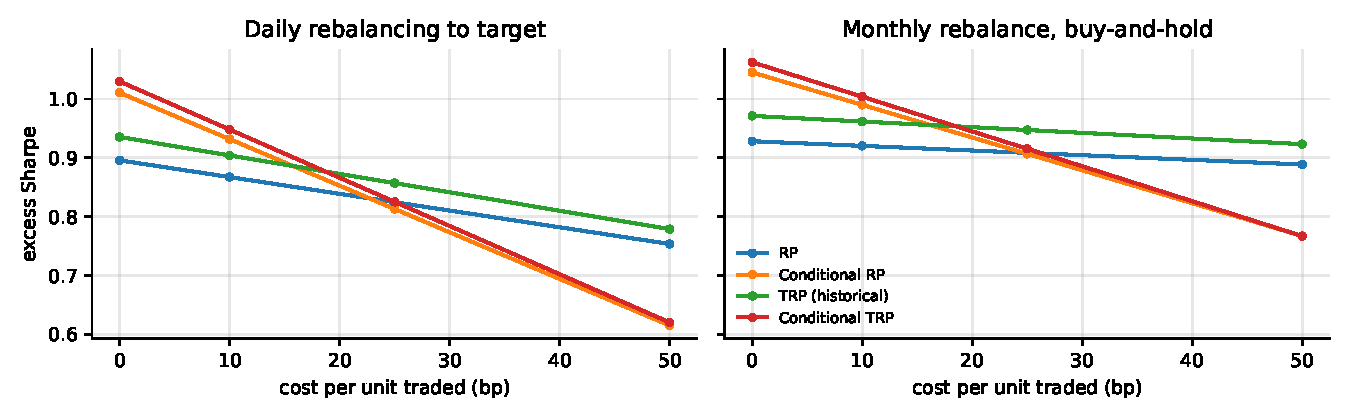
\includegraphics[width=0.92\textwidth]{figures/fig_trp_costs.pdf}
\caption{Excess Sharpe ratio against the transaction cost per unit traded, 2007-07 to 2026-10.}
\label{fig:costs}
\end{figure}

Table~\ref{tab:trp} and Figure~\ref{fig:costs} summarise the backtest from July 2007 to October 2026.

All figures below refer to monthly rebalancing with buy-and-hold; daily rebalancing gives the same
conclusions with higher turnover.

\emph{Replacing volatility by ES adds almost nothing.} Holding the scenarios fixed, the ES budget improves
the excess Sharpe ratio by 0.04 with unconditional scenarios and by 0.02 with conditional scenarios before
costs. Neither difference is significant (bootstrap 95\% intervals $[-0.02,0.11]$ and $[-0.06,0.09]$). Because ES and
volatility budgets have almost identical turnover, these differences hardly change with costs.

\emph{Conditioning on GARCH volatility is where the gross gain comes from, and costs remove it.}
Conditional RP improves on RP by 0.11 before costs (interval $[-0.07,0.30]$), almost the whole gain of conditional TRP
(0.13). But conditioning raises annual one-way turnover from 15\% to 95\% under monthly buy-and-hold, and
from 53\% to 136\% under daily rebalancing. At 10~bp the gain falls to about 0.07, at 25~bp it is zero, and
at 50~bp conditional strategies are about 0.12 \emph{worse} than plain RP. The conclusion is the same under
both execution rules; buy-and-hold has lower turnover and slightly higher net Sharpe ratios throughout.

Two further observations from the replication support this reading. In 2007--2012, the original
AllianceBernstein sample, TRP is slightly worse than RP in these data; the gross gains come from after 2013.
With a 99\% ES level, historical TRP deteriorates (only five tail observations in a 500-day window).

% ---------------------------------------------------------------------------
\section{Limitations}

\begin{itemize}
\item \textbf{Markets and sample.} Six asset classes, mostly Chinese and US, 2005--2026 for the allocation and
dependence tests. The conclusions are statements about this sample; tail behaviour in other markets or in
periods without a 2008-type crisis may differ.
\item \textbf{Asynchronous closes.} Weekly returns reduce but do not remove the bias from different closing
times. Tail dependence between Chinese and Western assets may be understated.
\item \textbf{Power.} Blocks of about 150 weekly observations contain roughly 15 decile exceedances per asset.
Weak tail dependence, for example in the stock--bond pair, may go undetected. The panel null controls the
size of the tests, not their power.
\item \textbf{Scope of the methods.} Only return-based ES is tested. The option-implied ES used in the
original tail-risk-parity proposal requires option data that do not exist for most Chinese assets. Static
copulas are fitted per window; dynamic copulas \citep{patton2006} and regime-dependent models are not
examined.
\item \textbf{Costs and performance measure.} Costs are a constant number of basis points per unit traded, with
no market impact and no differences between instruments. The excess Sharpe ratio is the primary criterion;
the replication also reports tail Sharpe ratios and drawdowns, which lead to the same ranking.
\item \textbf{Free data.} Index and ETF series come from free sources and were cross-checked (for example, two
ETF sources agree to within 0.08\% per day), but they are not vendor-grade.
\end{itemize}

% ---------------------------------------------------------------------------
\section{Conclusion}

Across the tests in this note, the information that changes risk forecasts and allocation outcomes is current
volatility and correlation. Single-parameter tail-dependence coefficients reproduce correlation almost
exactly. Tail dependence beyond correlation exists among risky assets but is invisible to the statistics used
in practice. Expected-shortfall budgeting adds little to volatility budgeting, and the part of tail risk parity
that does help before costs, conditioning on GARCH volatility, is consumed by its own turnover at realistic
costs. In long ES backtests the commonly used $Z_2$ threshold is uninformative and should be replaced by a
test with a proper null distribution. A practical implication is that tail-risk tools should be benchmarked
against correlation-matched nulls and volatility-conditioned alternatives, net of costs, before they are
credited with information of their own.

% ---------------------------------------------------------------------------
\bibliographystyle{plainnat}
\begin{thebibliography}{99}

\bibitem[Acerbi and Szekely(2014)]{acerbi2014}
Acerbi, C. and Szekely, B. (2014). Backtesting expected shortfall. \emph{Risk}, 27(11):76--81.

\bibitem[Alankar et~al.(2013)]{alankar2013}
Alankar, A., DePalma, M., and Scholes, M. (2013). An introduction to tail risk parity: balancing risk to
achieve downside protection. AllianceBernstein white paper.

\bibitem[Barone-Adesi et~al.(1999)]{baroneadesi1999}
Barone-Adesi, G., Giannopoulos, K., and Vosper, L. (1999). VaR without correlations for portfolios of
derivative securities. \emph{Journal of Futures Markets}, 19(5):583--602.

\bibitem[Christoffersen(1998)]{christoffersen1998}
Christoffersen, P.~F. (1998). Evaluating interval forecasts. \emph{International Economic Review},
39(4):841--862.

\bibitem[Demarta and McNeil(2005)]{demarta2005}
Demarta, S. and McNeil, A.~J. (2005). The $t$ copula and related copulas. \emph{International Statistical
Review}, 73(1):111--129.

\bibitem[Du and Escanciano(2017)]{duescanciano2017}
Du, Z. and Escanciano, J.~C. (2017). Backtesting expected shortfall: accounting for tail risk.
\emph{Management Science}, 63(4):940--958.

\bibitem[Embrechts et~al.(2002)]{embrechts2002}
Embrechts, P., McNeil, A.~J., and Straumann, D. (2002). Correlation and dependence in risk management:
properties and pitfalls. In Dempster, M. (ed.), \emph{Risk Management: Value at Risk and Beyond}, pages
176--223. Cambridge University Press.

\bibitem[Glosten et~al.(1993)]{glosten1993}
Glosten, L.~R., Jagannathan, R., and Runkle, D.~E. (1993). On the relation between the expected value and
the volatility of the nominal excess return on stocks. \emph{Journal of Finance}, 48(5):1779--1801.

\bibitem[Hall and Heyde(1980)]{hallheyde1980}
Hall, P. and Heyde, C.~C. (1980). \emph{Martingale Limit Theory and Its Application}. Academic Press.

\bibitem[Joe(1997)]{joe1997}
Joe, H. (1997). \emph{Multivariate Models and Dependence Concepts}. Chapman \& Hall.

\bibitem[Kupiec(1995)]{kupiec1995}
Kupiec, P.~H. (1995). Techniques for verifying the accuracy of risk measurement models. \emph{Journal of
Derivatives}, 3(2):73--84.

\bibitem[K{\"u}nsch(1989)]{kunsch1989}
K{\"u}nsch, H.~R. (1989). The jackknife and the bootstrap for general stationary observations.
\emph{Annals of Statistics}, 17(3):1217--1241.

\bibitem[Ledoit and Wolf(2008)]{ledoit2008}
Ledoit, O. and Wolf, M. (2008). Robust performance hypothesis testing with the Sharpe ratio.
\emph{Journal of Empirical Finance}, 15(5):850--859.

\bibitem[Maillard et~al.(2010)]{maillard2010}
Maillard, S., Roncalli, T., and Te{\"i}letche, J. (2010). The properties of equally weighted risk
contribution portfolios. \emph{Journal of Portfolio Management}, 36(4):60--70.

\bibitem[Mammen(1993)]{mammen1993}
Mammen, E. (1993). Bootstrap and wild bootstrap for high dimensional linear models. \emph{Annals of
Statistics}, 21(1):255--285.

\bibitem[Mausser and Romanko(2018)]{mausser2018}
Mausser, H. and Romanko, O. (2018). Long-only equal risk contribution portfolios for CVaR under discrete
distributions. \emph{Quantitative Finance}, 18(11):1927--1945.

\bibitem[McNeil and Frey(2000)]{mcneil2000}
McNeil, A.~J. and Frey, R. (2000). Estimation of tail-related risk measures for heteroscedastic financial
time series: an extreme value approach. \emph{Journal of Empirical Finance}, 7(3--4):271--300.

\bibitem[Patton(2006)]{patton2006}
Patton, A.~J. (2006). Modelling asymmetric exchange rate dependence. \emph{International Economic Review},
47(2):527--556.

\bibitem[Rockafellar and Uryasev(2000)]{rockafellar2000}
Rockafellar, R.~T. and Uryasev, S. (2000). Optimization of conditional value-at-risk. \emph{Journal of
Risk}, 2(3):21--41.

\bibitem[Spinu(2013)]{spinu2013}
Spinu, F. (2013). An algorithm for computing risk parity weights. SSRN Working Paper 2297383.

\bibitem[Wu(1986)]{wu1986}
Wu, C.~F.~J. (1986). Jackknife, bootstrap and other resampling methods in regression analysis.
\emph{Annals of Statistics}, 14(4):1261--1295.

\end{thebibliography}

\end{document}
